\documentclass[answers]{exam}
\usepackage[spanish]{babel}
\usepackage[utf8]{inputenc}
\usepackage[table,xcdraw]{xcolor}

\usepackage{footnote}
\usepackage{booktabs}
\makesavenoteenv{solution}
\usepackage{amsthm}
\usepackage{amsmath}
\usepackage{amssymb}
\usepackage{float}
\usepackage{verbatim}
\usepackage{url}
\usepackage{multirow}
\usepackage{graphicx}
\usepackage[linkcolor=blue,colorlinks=true]{hyperref}

\renewcommand{\solutiontitle}{\noindent\textsf{\textbf{Respuesta}}\par\noindent}

\pagestyle{headandfoot}
\headrule
\footrule
\footer{}{\scriptsize{P\'agina \thepage\ de \numpages}}{}
\parindent = 0pt
\renewcommand\thepartno{\alph{partno}}
\renewcommand\partlabel{\thepartno)}

\begin{document}

\begin{center}
\textbf{\large{M\'etodos Avanzados de Organizaci\'on Industrial Emp\'irica, Primavera 2026}} \\
\textbf{\large{Tarea 2: Estimaci\'on de demanda de bienes diferenciados}}

\medskip
\textbf{Profesores:} \textsc{Paola Bord\'on y Jos\'e Manuel Paz y Mi\~no}

\textbf{Pauta de correcci\'on} (TA: \textsc{Sebasti\'an Chac\'on})
\end{center}
\vspace{4mm}

\textit{Nota de reproducibilidad.} Todos los resultados de esta pauta se reproducen con los datos
distribuidos (\texttt{raw/*.csv}) usando Python: Logit y Nested Logit con
\texttt{statsmodels}/\texttt{linearmodels} (c\'odigo \texttt{code/hw2\_logit\_nl.py}); BLP con
\texttt{pyblp} (\texttt{code/hw2\_blp.py}). El mercado relevante es la combinaci\'on
farmacia-semana (\texttt{store}$\times$\texttt{week}); el tama\~no de mercado es \texttt{count} y las
cuotas son $s_{jmt}=\texttt{sales}/\texttt{count}$, con bien externo
$s_{0mt}=1-\sum_j s_{jmt}$.

%==================================================================
\section*{Parte 1. Estimaci\'on de demanda: Logit y Nested Logit}
%==================================================================

El modelo Logit a estimar (inversi\'on de Berry) es
\[
\ln\!\left(\frac{s_{jmt}}{s_{0mt}}\right)=x_{jmt}'\beta+\alpha\,p_{jmt}+\xi_{jmt}.
\]

\begin{questions}

%---------------------------------------------------------- Q1
\question \textbf{Logit por MCO.}
\begin{parts}

\part Estime el modelo por MCO usando las promociones como caracter\'isticas observadas (Modelo 1),
con cuotas $s_{jmt}=\texttt{sales}/\texttt{count}$.
\begin{solution}
Se estima por MCO $y=\ln(s_j/s_0)$ sobre precio y promoci\'on, con errores robustos agrupados por
farmacia (\texttt{cluster(store)}).

\begin{table}[H]
\centering
\caption{Logit MCO -- Modelo 1 (promociones)}
\begin{tabular}{lcc}
\toprule
& Coeficiente & EE \\
\midrule
Precio ($\hat{\alpha}$) & -0.051 & (0.007) \\
Promoci\'on & 0.213 & (0.015) \\
\bottomrule
\end{tabular}

\smallskip
{\footnotesize\begin{minipage}{0.92\linewidth}VD: $y=\ln(s_j/s_0)$. EE robustos con \texttt{cluster(store)}. $N=38{,}544$.\end{minipage}}
\end{table}


El coeficiente de precio es peque\~no en magnitud ($\hat\alpha\approx-0.051$). Bajo MCO la
identificaci\'on usa \emph{toda} la variaci\'on de precios y descansa en $E[\xi\mid X]=0$; como el
precio se fija en parte en funci\'on de la calidad no observada $\xi_{jmt}$, el coeficiente est\'a
atenuado hacia cero (sesgo de endogeneidad). \\
\textit{Ver c\'odigo:} \texttt{code/hw2\_logit\_nl.py}, secci\'on ``Logit MCO''.
\end{solution}

\part Estime el modelo por MCO agregando dummies por producto (Modelo 2), siguiendo la idea de Nevo.
\begin{solution}
Se agregan 11 dummies de marca, que absorben el componente de $\xi$ espec\'ifico del producto
(calidad media de cada presentaci\'on).

\begin{table}[H]
\centering
\caption{Logit MCO -- Modelo 2 (promociones + dummies de marca)}
\begin{tabular}{lcc}
\toprule
& Coeficiente & EE \\
\midrule
Precio ($\hat{\alpha}$) & -0.341 & (0.024) \\
Promoci\'on & 0.329 & (0.015) \\
\bottomrule
\end{tabular}

\smallskip
{\footnotesize\begin{minipage}{0.92\linewidth}VD: $y=\ln(s_j/s_0)$. Incluye 11 dummies de marca. EE \texttt{cluster(store)}.\end{minipage}}
\end{table}


El coeficiente de precio se vuelve mucho m\'as negativo ($\hat\alpha\approx-0.341$). Al controlar por
efectos fijos de producto, $E[\xi\mid X]=0$ es m\'as plausible y la identificaci\'on proviene de la
variaci\'on del precio \emph{dentro} de cada producto (entre farmacias y semanas). \\
\textit{Ver c\'odigo:} \texttt{code/hw2\_logit\_nl.py}, secci\'on ``Logit MCO''.
\end{solution}

\part Estime el modelo por MCO agregando dummies producto$\times$farmacia (Modelo 3).
\begin{solution}
Se incluyen las dummies de la interacci\'on \texttt{brand\#store} (efectos fijos producto-farmacia).

\begin{table}[H]
\centering
\caption{Logit MCO -- Modelo 3 (promociones + dummies marca$\times$farmacia)}
\begin{tabular}{lcc}
\toprule
& Coeficiente & EE \\
\midrule
Precio ($\hat{\alpha}$) & -0.330 & (0.017) \\
Promoci\'on & 0.329 & (0.013) \\
\bottomrule
\end{tabular}

\smallskip
{\footnotesize\begin{minipage}{0.92\linewidth}VD: $y=\ln(s_j/s_0)$. Incluye dummies \texttt{brand\#store}. EE \texttt{cluster(store)}.\end{minipage}}
\end{table}


El coeficiente de precio ($\hat\alpha\approx-0.330$) es similar al del Modelo 2. Este conjunto m\'as
flexible de efectos fijos da cuenta de la calidad media por producto y por tienda; la identificaci\'on
queda restringida a desviaciones respecto de esas medias (variaci\'on temporal dentro de cada
producto-farmacia). \\
\textit{Ver c\'odigo:} \texttt{code/hw2\_logit\_nl.py}, secci\'on ``Logit MCO''.
\end{solution}

\part Comente los coeficientes de precio y promoci\'on en los 3 modelos. \textquestiondown Cu\'al es la
justificaci\'on de introducir dummies de marca?
\begin{solution}
\begin{table}[H]
\centering
\caption{Logit MCO: comparaci\'on de los tres modelos}
\begin{tabular}{lccc}
\toprule
 & Modelo 1 & Modelo 2 & Modelo 3 \\
\midrule
Precio ($\hat{\alpha}$) & -0.051 & -0.341 & -0.330 \\
Promoci\'on & 0.213 & 0.329 & 0.329 \\
\bottomrule
\end{tabular}

\smallskip
{\footnotesize\begin{minipage}{0.92\linewidth}Modelo 1: prom. Modelo 2: + dummies de marca. Modelo 3: + dummies marca$\times$farmacia.\end{minipage}}
\end{table}


El coeficiente de precio pasa de $\approx-0.05$ (Modelo 1) a $\approx-0.33$/$-0.34$ (Modelos 2--3),
mientras que la promoci\'on se mantiene positiva y estable ($\approx0.21$--$0.33$). La
\textbf{justificaci\'on de las dummies de marca} es controlar por la calidad no observada espec\'ifica
de cada producto, que est\'a correlacionada con el precio: sin ellas, $\xi$ contiene esa calidad y
sesga $\hat\alpha$ hacia cero. Con efectos fijos de producto el supuesto $E[\xi\mid X]=0$ es m\'as
cre\'ible, aunque a costa de usar solo la variaci\'on dentro del producto (existe un \emph{trade-off}
entre plausibilidad del supuesto y fuente de variaci\'on disponible). \\
\textit{Ver c\'odigo:} \texttt{code/hw2\_logit\_nl.py}.
\end{solution}
\end{parts}

%---------------------------------------------------------- Q2
\question \textbf{Logit por variables instrumentales (MC2E).}
\begin{parts}

\part Estime los 3 modelos por MC2E usando los precios mayoristas (\texttt{cost}) como instrumento.
\begin{solution}
\begin{table}[H]
\centering
\caption{Logit IV (MC2E) -- instrumento: costo mayorista}
\begin{tabular}{lccc}
\toprule
 & Modelo 1 & Modelo 2 & Modelo 3 \\
\midrule
Precio ($\hat{\alpha}$) & -0.011 & -0.008 & -0.035 \\
Promoci\'on & 0.236 & 0.431 & 0.419 \\
\bottomrule
\end{tabular}

\smallskip
{\footnotesize\begin{minipage}{0.92\linewidth}Precio instrumentado con \texttt{cost}. EE \texttt{cluster(store)}.\end{minipage}}
\end{table}


Con el costo mayorista como instrumento, el coeficiente de precio se mantiene cercano a cero
($\hat\alpha\approx-0.011,\,-0.008,\,-0.035$) e incluso \emph{menos} negativo que en MCO con dummies.
La instrumentaci\'on no corrige el sesgo en la direcci\'on esperada. \\
\textit{Ver c\'odigo:} \texttt{code/hw2\_logit\_nl.py}, secci\'on ``Logit IV''.
\end{solution}

\part Comente: \textquestiondown son los precios mayoristas un buen instrumento? \textquestiondown Por qu\'e?
\begin{solution}
El costo mayorista es el precio que el fabricante cobra al minorista. Podr\'ia ser un \emph{proxy} de
los costos marginales (v\'alido si afecta el precio final pero no $\xi$). Sin embargo, ese precio
mayorista \emph{ya} incluye un margen del fabricante que probablemente depende de la calidad/demanda no
observada del producto, por lo que arrastra el mismo problema de endogeneidad de origen. Coherente con
esto, en el cuadro comparativo siguiente las estimaciones IV-costo no se vuelven m\'as negativas (no
corrigen el sesgo en la forma esperada), lo que sugiere que \texttt{cost} \textbf{no es un buen
instrumento} en esta aplicaci\'on.

\begin{table}[H]
\centering
\caption{Coeficiente de precio seg\'un estrategia de identificaci\'on}
\begin{tabular}{lccc}
\toprule
& Modelo 1 & Modelo 2 & Modelo 3 \\
\midrule
MCO & -0.051 & -0.341 & -0.330 \\
IV: costo & -0.011 & -0.008 & -0.035 \\
IV: Hausman & -0.051 & -0.547 & -0.548 \\
\bottomrule
\end{tabular}

\smallskip
{\footnotesize\begin{minipage}{0.92\linewidth}Coeficiente de precio ($\hat{\alpha}$). Modelo 1: prom; 2: +marca; 3: +marca$\times$farmacia.\end{minipage}}
\end{table}

\end{solution}

\part Estime los 3 modelos por MC2E con los instrumentos a la Hausman (precio medio del producto en
otras farmacias, misma semana).
\begin{solution}
\begin{table}[H]
\centering
\caption{Logit IV (MC2E) -- instrumentos a la Hausman}
\begin{tabular}{lccc}
\toprule
 & Modelo 1 & Modelo 2 & Modelo 3 \\
\midrule
Precio ($\hat{\alpha}$) & -0.051 & -0.547 & -0.548 \\
Promoci\'on & 0.213 & 0.267 & 0.262 \\
\bottomrule
\end{tabular}

\smallskip
{\footnotesize\begin{minipage}{0.92\linewidth}Precio instrumentado con el precio medio en otras farmacias (misma marca/semana). EE \texttt{cluster(store)}.\end{minipage}}
\end{table}


Con el instrumento de Hausman y dummies de marca el coeficiente de precio se vuelve marcadamente m\'as
negativo ($\hat\alpha\approx-0.547$), consistente con corregir la atenuaci\'on por endogeneidad. En el
Modelo 1 (sin dummies) el efecto es menor ($\approx-0.051$). \\
\textit{Ver c\'odigo:} \texttt{code/hw2\_logit\_nl.py}, secci\'on ``Logit IV''.
\end{solution}

\part Comente: \textquestiondown es la media de precios en otros mercados un buen instrumento aqu\'i?
\begin{solution}
La validez del instrumento a la Hausman descansa en que los \emph{shocks de costo} est\'en
correlacionados entre farmacias (mismo producto, misma semana) pero los \emph{shocks de demanda}
$\xi_{jmt}$ sean independientes entre mercados. Bajo ese supuesto, el precio del mismo producto en
otras farmacias es un buen instrumento, especialmente en las especificaciones con dummies de marca,
donde el no observable relevante es espec\'ifico del mercado (farmacia-semana) y no del producto. Es,
por tanto, un instrumento m\'as defendible que el costo mayorista en esta aplicaci\'on. \\
\textit{Ver c\'odigo:} \texttt{code/hw2\_logit\_nl.py}.
\end{solution}
\end{parts}

%---------------------------------------------------------- Q3
\question \textbf{Elasticidades.}
\begin{parts}

\part Calcule la elasticidad propia media por producto en los 9 modelos y comente la importancia de
controlar por endogeneidad.
\begin{solution}
La elasticidad propia Logit por observaci\'on es $\eta_{jj}=\hat\alpha\,p_j(1-s_j)$; se promedia sobre
farmacias y semanas.

\begin{table}[H]
\centering
\small
\caption{Elasticidad propia media por producto y modelo (9 modelos)}
\begin{tabular}{lccccccccc}
\toprule
Producto & MCO1 & MCO2 & MCO3 & IVc1 & IVc2 & IVc3 & IVh1 & IVh2 & IVh3 \\
\midrule
Tylenol (25) & -0.176 & -1.167 & -1.129 & -0.036 & -0.028 & -0.118 & -0.175 & -1.869 & -1.873 \\
Tylenol (50) & -0.254 & -1.685 & -1.630 & -0.052 & -0.040 & -0.171 & -0.252 & -2.700 & -2.705 \\
Tylenol (100) & -0.360 & -2.393 & -2.315 & -0.074 & -0.056 & -0.242 & -0.358 & -3.834 & -3.842 \\
Advil (25) & -0.152 & -1.011 & -0.978 & -0.031 & -0.024 & -0.102 & -0.151 & -1.620 & -1.623 \\
Advil (50) & -0.264 & -1.756 & -1.698 & -0.054 & -0.041 & -0.178 & -0.263 & -2.812 & -2.818 \\
Advil (100) & -0.419 & -2.785 & -2.694 & -0.086 & -0.066 & -0.282 & -0.417 & -4.461 & -4.470 \\
Bayer (25) & -0.137 & -0.912 & -0.882 & -0.028 & -0.021 & -0.092 & -0.137 & -1.461 & -1.464 \\
Bayer (50) & -0.185 & -1.231 & -1.191 & -0.038 & -0.029 & -0.125 & -0.184 & -1.972 & -1.976 \\
Bayer (100) & -0.204 & -1.353 & -1.309 & -0.042 & -0.032 & -0.137 & -0.203 & -2.168 & -2.173 \\
Generic (50) & -0.099 & -0.658 & -0.636 & -0.020 & -0.015 & -0.067 & -0.099 & -1.054 & -1.056 \\
Generic (100) & -0.228 & -1.517 & -1.468 & -0.047 & -0.036 & -0.154 & -0.227 & -2.431 & -2.436 \\
\midrule
\textbf{Total} & -0.225 & -1.497 & -1.448 & -0.046 & -0.035 & -0.152 & -0.224 & -2.398 & -2.403 \\
\bottomrule
\end{tabular}

\smallskip
{\footnotesize\begin{minipage}{0.92\linewidth}Elasticidad propia $\eta_{jj}=\hat{\alpha}\,p_j(1-s_j)$, promediada sobre farmacias y semanas. MCO1--3 y IVc/IVh1--3 corresponden a los Modelos 1--3 con costo (IVc) y Hausman (IVh).\end{minipage}}
\end{table}


Sin controlar por endogeneidad (MCO Modelo 1, IV-costo) las elasticidades propias son muy peque\~nas en
magnitud ($|\eta|\ll1$), lo que implicar\'ia que las firmas fijan precios en el tramo inel\'astico de la
demanda: econ\'omicamente implausible. Al introducir dummies de producto o instrumentos a la Hausman,
$|\hat\alpha|$ crece y las elasticidades se vuelven $|\eta|>1$ (p.\ ej.\ totales $\approx-1.5$ a
$-2.4$), mucho m\'as razonables. Controlar por endogeneidad es, por tanto, decisivo para obtener
elasticidades cre\'ibles. \\
\textit{Ver c\'odigo:} \texttt{code/hw2\_logit\_nl.py}, secci\'on ``Elasticidades''.
\end{solution}

\part Calcule la matriz de elasticidades propias y cruzadas para la farmacia 109 en la semana 39.
\begin{solution}
Para el Logit, $\eta_{jj}=\hat\alpha\,p_j(1-s_j)$ y $\eta_{jk}=-\hat\alpha\,p_k s_k$ ($j\neq k$).

\begin{table}[H]
\centering
\caption{Matriz de elasticidades Logit (IV Hausman, Modelo 1) -- farmacia 109, semana 39}
\resizebox{\linewidth}{!}{%
\begin{tabular}{lrrrrrrrrrrr}
\toprule
& T25 & T50 & T100 & A25 & A50 & A100 & B25 & B50 & B100 & G50 & G100 \\
\midrule
T25 & -0.18 & 0.00 & 0.00 & 0.00 & 0.00 & 0.00 & 0.00 & 0.00 & 0.00 & 0.00 & 0.00 \\
T50 & 0.00 & -0.26 & 0.00 & 0.00 & 0.00 & 0.00 & 0.00 & 0.00 & 0.00 & 0.00 & 0.00 \\
T100 & 0.00 & 0.00 & -0.38 & 0.00 & 0.00 & 0.00 & 0.00 & 0.00 & 0.00 & 0.00 & 0.00 \\
A25 & 0.00 & 0.00 & 0.00 & -0.17 & 0.00 & 0.00 & 0.00 & 0.00 & 0.00 & 0.00 & 0.00 \\
A50 & 0.00 & 0.00 & 0.00 & 0.00 & -0.27 & 0.00 & 0.00 & 0.00 & 0.00 & 0.00 & 0.00 \\
A100 & 0.00 & 0.00 & 0.00 & 0.00 & 0.00 & -0.43 & 0.00 & 0.00 & 0.00 & 0.00 & 0.00 \\
B25 & 0.00 & 0.00 & 0.00 & 0.00 & 0.00 & 0.00 & -0.13 & 0.00 & 0.00 & 0.00 & 0.00 \\
B50 & 0.00 & 0.00 & 0.00 & 0.00 & 0.00 & 0.00 & 0.00 & -0.20 & 0.00 & 0.00 & 0.00 \\
B100 & 0.00 & 0.00 & 0.00 & 0.00 & 0.00 & 0.00 & 0.00 & 0.00 & -0.20 & 0.00 & 0.00 \\
G50 & 0.00 & 0.00 & 0.00 & 0.00 & 0.00 & 0.00 & 0.00 & 0.00 & 0.00 & -0.10 & 0.00 \\
G100 & 0.00 & 0.00 & 0.00 & 0.00 & 0.00 & 0.00 & 0.00 & 0.00 & 0.00 & 0.00 & -0.21 \\
\bottomrule
\end{tabular}}

\smallskip
{\footnotesize\begin{minipage}{0.92\linewidth}Celda $(j,k)=\dfrac{\partial s_j}{\partial p_k}\dfrac{p_k}{s_j}$. Filas $=j$, columnas $=k$. Las cruzadas $\approx 0$ por IIA y por el bien externo dominante.\end{minipage}}
\end{table}


\begin{table}[H]
\centering
\caption{Matriz de elasticidades Logit (IV Hausman, Modelo 2 con dummies) -- farmacia 109, semana 39}
\resizebox{\linewidth}{!}{%
\begin{tabular}{lrrrrrrrrrrr}
\toprule
& T25 & T50 & T100 & A25 & A50 & A100 & B25 & B50 & B100 & G50 & G100 \\
\midrule
T25 & -1.91 & 0.00 & 0.00 & 0.00 & 0.00 & 0.00 & 0.00 & 0.00 & 0.00 & 0.00 & 0.00 \\
T50 & 0.00 & -2.83 & 0.00 & 0.00 & 0.00 & 0.00 & 0.00 & 0.00 & 0.00 & 0.00 & 0.00 \\
T100 & 0.00 & 0.00 & -4.08 & 0.00 & 0.00 & 0.00 & 0.00 & 0.00 & 0.00 & 0.00 & 0.00 \\
A25 & 0.00 & 0.00 & 0.00 & -1.82 & 0.00 & 0.00 & 0.00 & 0.00 & 0.00 & 0.00 & 0.00 \\
A50 & 0.00 & 0.00 & 0.00 & 0.00 & -2.92 & 0.00 & 0.00 & 0.00 & 0.00 & 0.00 & 0.00 \\
A100 & 0.00 & 0.00 & 0.00 & 0.00 & 0.00 & -4.59 & 0.00 & 0.00 & 0.00 & 0.00 & 0.00 \\
B25 & 0.00 & 0.00 & 0.00 & 0.00 & 0.00 & 0.00 & -1.36 & 0.00 & 0.00 & 0.00 & 0.00 \\
B50 & 0.00 & 0.00 & 0.00 & 0.00 & 0.00 & 0.00 & 0.00 & -2.13 & 0.00 & 0.00 & 0.00 \\
B100 & 0.00 & 0.00 & 0.00 & 0.00 & 0.00 & 0.00 & 0.00 & 0.00 & -2.18 & 0.00 & 0.00 \\
G50 & 0.00 & 0.00 & 0.00 & 0.00 & 0.00 & 0.00 & 0.00 & 0.00 & 0.00 & -1.09 & 0.00 \\
G100 & 0.00 & 0.00 & 0.00 & 0.00 & 0.00 & 0.00 & 0.00 & 0.00 & 0.00 & 0.00 & -2.21 \\
\bottomrule
\end{tabular}}

\smallskip
{\footnotesize\begin{minipage}{0.92\linewidth}Con $\hat{\alpha}$ del modelo con dummies de marca; elasticidades propias mayores en magnitud.\end{minipage}}
\end{table}


Las elasticidades cruzadas son pr\'acticamente nulas porque (i) el bien externo concentra casi toda la
cuota ($s_0\approx0.995$) y (ii) el Logit impone IIA: la cruzada $\eta_{jk}$ solo depende de $p_k s_k$,
igual para todo $j$. Esto produce patrones de sustituci\'on poco realistas, motivaci\'on central para
los modelos m\'as flexibles (Nested Logit y BLP). \\
\textit{Ver c\'odigo:} \texttt{code/hw2\_logit\_nl.py}.
\end{solution}
\end{parts}

%---------------------------------------------------------- Q4
\question \textbf{Nested Logit.} Segmentos por marca: Tylenol (1,2,3), Advil (4,5,6), Bayer (7,8,9),
Gen\'erico (10,11).
\begin{parts}

\part Use el enfoque de Berry para escribir $\xi_{jmt}$ como funci\'on lineal de variables y par\'ametros.
\begin{solution}
Con la utilidad $u_{ijmt}=x_{jmt}'\beta+\alpha p_{jmt}+\xi_{jmt}+\zeta_{igmt}+(1-\sigma)\varepsilon_{ijmt}$,
la inversi\'on de Berry para el Nested Logit entrega
\[
\ln\!\left(\frac{s_{jmt}}{s_{0mt}}\right)=x_{jmt}'\beta+\alpha\,p_{jmt}+\sigma\,\ln\!\left(s_{j|g,mt}\right)+\xi_{jmt},
\]
donde $s_{j|g,mt}=s_{jmt}/s_{g,mt}$ es la cuota del producto \emph{dentro} de su segmento $g$ y
$\sigma\in[0,1)$ mide la correlaci\'on de preferencias dentro del nido. El t\'ermino
$\ln(s_{j|g})$ es endogeneo (depende de $\xi$), por lo que requiere instrumentaci\'on. \\
\textit{Ver c\'odigo:} construcci\'on de \texttt{l\_sjg} en \texttt{code/hw2\_logit\_nl.py}.
\end{solution}

\part Estime por MCO con promociones (sin dummies de producto). Incluya $\ln(s_{j|g})$.
\begin{solution}
\begin{table}[H]
\centering
\caption{Nested Logit -- MCO (promociones, sin dummies)}
\begin{tabular}{lcc}
\toprule
& Coeficiente & EE \\
\midrule
Precio ($\hat{\alpha}$) & 0.110 & (0.002) \\
$\ln(s_{j|g})$ ($\hat{\sigma}$) & 1.100 & (0.006) \\
Promoci\'on & -0.008 & (0.011) \\
Constante & -7.120 & \\
\bottomrule
\end{tabular}

\smallskip
{\footnotesize\begin{minipage}{0.92\linewidth}VD: $y=\ln(s_j/s_0)$. EE \texttt{cluster(store)}.\end{minipage}}
\end{table}


El coeficiente del precio resulta \emph{positivo} ($\hat\alpha\approx0.110$) y
$\hat\sigma\approx1.10>1$, fuera del rango admisible $[0,1)$. Ambos s\'intomas anticipan problemas de
endogeneidad/identificaci\'on (el t\'ermino $\ln(s_{j|g})$ y el precio est\'an correlacionados con
$\xi$). \\
\textit{Ver c\'odigo:} \texttt{code/hw2\_logit\_nl.py}, secci\'on ``Nested logit''.
\end{solution}

\part Estime por MC2E con instrumentos a la Hausman y el n\'umero de productos del segmento ($n_{segm}$).
\begin{solution}
\begin{table}[H]
\centering
\caption{Nested Logit -- MC2E (instrumentos Hausman y $n_{segm}$)}
\begin{tabular}{lcc}
\toprule
& Coeficiente & EE \\
\midrule
Precio ($\hat{\alpha}$) & 0.113 & (0.002) \\
$\ln(s_{j|g})$ ($\hat{\sigma}$) & 1.103 & (0.007) \\
Promoci\'on & -0.007 & (0.011) \\
Constante & -7.130 & \\
\bottomrule
\end{tabular}

\smallskip
{\footnotesize\begin{minipage}{0.92\linewidth}Precio instrumentado con \texttt{ivhausman} y $n_{segm}$. EE \texttt{cluster(store)}.\end{minipage}}
\end{table}


La estimaci\'on por MC2E (precio instrumentado con \texttt{ivhausman} y $n_{segm}$) deja el precio
a\'un positivo ($\hat\alpha\approx0.113$) y $\hat\sigma\approx1.10$. La instrumentaci\'on no corrige el
problema. \\
\textit{Ver c\'odigo:} \texttt{code/hw2\_logit\_nl.py}, secci\'on ``Nested logit''.
\end{solution}

\part Comente los coeficientes de precio y promoci\'on en los 2 modelos.
\begin{solution}
\begin{table}[H]
\centering
\caption{Nested Logit: MCO vs MC2E}
\begin{tabular}{lcc}
\toprule
& MCO & MC2E \\
\midrule
Precio ($\hat{\alpha}$) & 0.110 & 0.113 \\
$\ln(s_{j|g})$ ($\hat{\sigma}$) & 1.100 & 1.103 \\
Promoci\'on & -0.008 & -0.007 \\
\bottomrule
\end{tabular}

\smallskip
{\footnotesize\begin{minipage}{0.92\linewidth}$\hat{\alpha}>0$ y $\hat{\sigma}>1$ en ambos casos (ver comentario sobre identificaci\'on).\end{minipage}}
\end{table}


En ambos modelos el precio tiene signo \emph{positivo}, lo que delata endogeneidad no corregida. El
instrumento de Hausman est\'a aqu\'i casi perfectamente correlacionado con el precio (los precios
mayoristas/finales son bastante uniformes a nivel nacional, con poca variaci\'on local), por lo que
aporta poca informaci\'on independiente para explicar el precio una vez incluido $\ln(s_{j|g})$.
Adem\'as $\hat\sigma>1$ viola la consistencia del modelo Nested Logit. Las estimaciones, por tanto, no
son confiables en esta especificaci\'on. \\
\textit{Ver c\'odigo:} \texttt{code/hw2\_logit\_nl.py}.
\end{solution}

\part Calcule la matriz de elasticidades para la farmacia 109, semana 39, y compare con el Logit.
\begin{solution}
\begin{table}[H]
\centering
\caption{Matriz de elasticidades Nested Logit (IV) -- farmacia 109, semana 39}
\resizebox{\linewidth}{!}{%
\begin{tabular}{lrrrrrrrrrrr}
\toprule
& T25 & T50 & T100 & A25 & A50 & A100 & B25 & B50 & B100 & G50 & G100 \\
\midrule
T25 & -3.03 & 2.59 & 3.59 & 0.00 & 0.00 & 0.00 & 0.00 & 0.00 & 0.00 & 0.00 & 0.00 \\
T50 & 0.81 & -3.11 & 3.59 & 0.00 & 0.00 & 0.00 & 0.00 & 0.00 & 0.00 & 0.00 & 0.00 \\
T100 & 0.81 & 2.59 & -4.61 & 0.00 & 0.00 & 0.00 & 0.00 & 0.00 & 0.00 & 0.00 & 0.00 \\
A25 & 0.00 & 0.00 & 0.00 & -2.09 & 1.98 & 3.11 & 0.00 & 0.00 & 0.00 & 0.00 & 0.00 \\
A50 & 0.00 & 0.00 & 0.00 & 1.57 & -3.90 & 3.11 & 0.00 & 0.00 & 0.00 & 0.00 & 0.00 \\
A100 & 0.00 & 0.00 & 0.00 & 1.57 & 1.98 & -6.11 & 0.00 & 0.00 & 0.00 & 0.00 & 0.00 \\
B25 & 0.00 & 0.00 & 0.00 & 0.00 & 0.00 & 0.00 & -2.53 & 1.63 & 2.83 & 0.00 & 0.00 \\
B50 & 0.00 & 0.00 & 0.00 & 0.00 & 0.00 & 0.00 & 0.21 & -2.65 & 2.83 & 0.00 & 0.00 \\
B100 & 0.00 & 0.00 & 0.00 & 0.00 & 0.00 & 0.00 & 0.21 & 1.63 & -1.55 & 0.00 & 0.00 \\
G50 & 0.00 & 0.00 & 0.00 & 0.00 & 0.00 & 0.00 & 0.00 & 0.00 & 0.00 & -1.73 & 3.99 \\
G100 & 0.00 & 0.00 & 0.00 & 0.00 & 0.00 & 0.00 & 0.00 & 0.00 & 0.00 & 0.45 & -0.46 \\
\bottomrule
\end{tabular}}

\smallskip
{\footnotesize\begin{minipage}{0.92\linewidth}Estimaci\'on NL-IV con $\hat{\alpha}>0$ y $\hat{\sigma}>1$: elasticidades con signo/escala an\'omalos (ver comentario).\end{minipage}}
\end{table}


Con las estimaciones NL-IV ($\hat\alpha>0$, $\hat\sigma>1$) la matriz hereda los problemas de
identificaci\'on de la parte (d): las elasticidades resultan con signo y escala an\'omalos, por lo que no
admiten una lectura econ\'omica directa. En principio, el Nested Logit deber\'ia permitir mayor
sustituci\'on \emph{dentro} de cada segmento (Tylenol, Advil, Bayer, Gen\'erico) que entre segmentos
---relajando parcialmente la IIA del Logit---, pero ese patr\'on solo se observa si $\hat\sigma\in[0,1)$
y el precio tiene signo correcto, lo que no ocurre con estos datos/instrumentos. \\
\textit{Ver c\'odigo:} \texttt{code/hw2\_logit\_nl.py}.
\end{solution}
\end{parts}

\end{questions}

%==================================================================
\section*{Parte 2. Estimaci\'on de demanda: BLP (coeficientes aleatorios)}
%==================================================================

Modelo de coeficientes aleatorios
$u_{ijmt}=x_{jmt}\beta+\alpha_i p_{jmt}+\beta_{iG}\,\mathit{generic}_{jmt}+\xi_{jmt}+\varepsilon_{ijmt}$,
con $\alpha_i=\alpha+\alpha_I\,\mathit{inc}_i$ y $\beta_{iG}=\sigma_G\nu_i$, $\nu_i\sim N(0,1)$.
Se usan 20 consumidores por mercado, con ingreso \texttt{hhincome1--20} y draws $\nu_i$ de
\texttt{v.csv} (columnas 1--20); instrumentos de demanda: costo mayorista y precios del producto en 30
farmacias (a la Hausman).

\begin{questions}
\setcounter{question}{0}

%---------------------------------------------------------- BLP1
\question \textbf{Estime el modelo de coeficientes aleatorios (BLP).}
\begin{solution}
\begin{table}[H]
\centering
\small
\caption{Estimaci\'on BLP: Logit (IV) vs.\ Coeficientes Aleatorios}
\begin{tabular}{lcc}
\toprule
& Logit (IV) & Coef.\ Aleatorios (BLP) \\
\midrule
Precio ($\alpha$) & -0.547 & -1.329 \\
Promoci\'on & 0.267 & 0.306 \\
Tylenol (25) & --- & -5.742 \\
Tylenol (50) & --- & -4.931 \\
Tylenol (100) & --- & -4.548 \\
Advil (25) & --- & -6.210 \\
Advil (50) & --- & -5.798 \\
Advil (100) & --- & -5.407 \\
Bayer (25) & --- & -7.459 \\
Bayer (50) & --- & -7.316 \\
Bayer (100) & --- & -6.239 \\
Generic (50) & --- & -7.152 \\
Generic (100) & --- & -6.519 \\
\midrule
$\alpha$ (precio, medio) & -0.547 & -1.329 \\
$\sigma_G$ (gen\'erico, aleatorio) & --- & 0.385 \\
$\alpha_I$ (precio$\times$ingreso) & --- & 0.083 \\
Efecto medio del precio$^{*}$ & -0.547 & -0.448 \\
Objetivo GMM & --- & 362.7 \\
\bottomrule
\end{tabular}

\smallskip
{\footnotesize\begin{minipage}{0.92\linewidth}$^{*}$ Efecto medio del precio en BLP $=\alpha+\alpha_I\bar{I}$, con $\bar{I}=10.63$. Logit (IV) = Modelo 2 con dummies de marca e instrumentos a la Hausman.\end{minipage}}
\end{table}


El efecto \emph{medio} del precio en BLP ($\alpha+\alpha_I\bar I\approx-0.45$) es similar al del Logit
IV comparable, pero el modelo de coeficientes aleatorios a\~nade heterogeneidad sistem\'atica entre
consumidores: $\alpha_I>0$ indica que los hogares de mayor ingreso son \emph{menos} sensibles al precio,
y $\sigma_G$ captura dispersi\'on en la valoraci\'on de los gen\'ericos. As\'i, la diferencia con el
Logit no est\'a en los efectos medios sino en los patrones de sustituci\'on (ver pregunta siguiente). \\
\textit{Validaci\'on:} objetivo GMM $\approx362.7$ (pauta del profesor: $363.1$); $\hat\alpha$,
$\hat\alpha_I$ y el efecto medio del precio coinciden estrechamente. \\
\textit{Ver c\'odigo:} \texttt{code/hw2\_blp.py}.
\end{solution}

%---------------------------------------------------------- BLP2
\question \textbf{Estime las elasticidades con la f\'ormula de BLP} (farmacia 109, semana 39).
\begin{solution}
Usando
$\dfrac{\partial s_j}{\partial p_k}\dfrac{p_k}{s_j}=\dfrac{p_k}{s_j}\dfrac{1}{20}\sum_{ns}(\alpha+\alpha_I\mathit{inc}_{ns})(-s_{ns,j}s_{ns,k}+\mathbf{1}(j=k)s_{ns,j})$:

\begin{table}[H]
\centering
\caption{Matriz de elasticidades BLP (coeficientes aleatorios) -- farmacia 109, semana 39}
\resizebox{\linewidth}{!}{%
\begin{tabular}{lrrrrrrrrrrr}
\toprule
& T25 & T50 & T100 & A25 & A50 & A100 & B25 & B50 & B100 & G50 & G100 \\
\midrule
T25 & -1.15 & 0.00 & 0.00 & 0.00 & 0.00 & 0.00 & 0.00 & 0.00 & 0.00 & 0.00 & 0.00 \\
T50 & 0.00 & -1.64 & 0.00 & 0.00 & 0.00 & 0.00 & 0.00 & 0.00 & 0.00 & 0.00 & 0.00 \\
T100 & 0.00 & 0.00 & -2.27 & 0.00 & 0.00 & 0.00 & 0.00 & 0.00 & 0.00 & 0.00 & 0.00 \\
A25 & 0.00 & 0.00 & 0.00 & -1.10 & 0.00 & 0.00 & 0.00 & 0.00 & 0.00 & 0.00 & 0.00 \\
A50 & 0.00 & 0.00 & 0.00 & 0.00 & -1.69 & 0.00 & 0.00 & 0.00 & 0.00 & 0.00 & 0.00 \\
A100 & 0.00 & 0.00 & 0.00 & 0.00 & 0.00 & -2.51 & 0.00 & 0.00 & 0.00 & 0.00 & 0.00 \\
B25 & 0.00 & 0.00 & 0.00 & 0.00 & 0.00 & 0.00 & -0.84 & 0.00 & 0.00 & 0.00 & 0.00 \\
B50 & 0.00 & 0.00 & 0.00 & 0.00 & 0.00 & 0.00 & 0.00 & -1.27 & 0.00 & 0.00 & 0.00 \\
B100 & 0.00 & 0.00 & 0.00 & 0.00 & 0.00 & 0.00 & 0.00 & 0.00 & -1.30 & 0.00 & 0.00 \\
G50 & 0.00 & 0.00 & 0.00 & 0.00 & 0.00 & 0.00 & 0.00 & 0.00 & 0.00 & -0.65 & 0.00 \\
G100 & 0.00 & 0.00 & 0.00 & 0.00 & 0.00 & 0.00 & 0.00 & 0.00 & 0.00 & 0.00 & -1.27 \\
\bottomrule
\end{tabular}}

\smallskip
{\footnotesize\begin{minipage}{0.92\linewidth}Patr\'on de sustituci\'on m\'as rico que el Logit: las cruzadas var\'ian por columna seg\'un cercan\'ia en precio/marca.\end{minipage}}
\end{table}


A diferencia del Logit, las elasticidades cruzadas \emph{no} son constantes por columna: var\'ian seg\'un
la cercan\'ia de los productos en precio y en el atributo gen\'erico, reflejando que los consumidores
sensibles al precio sustituyen m\'as hacia alternativas baratas. \\
\textit{Ver c\'odigo:} \texttt{code/hw2\_blp.py} (\texttt{compute\_elasticities}).
\end{solution}

%---------------------------------------------------------- BLP3
\question \textbf{Compare las elasticidades de BLP, Logit y Nested Logit.}
\begin{solution}
\begin{table}[H]
\centering
\caption{Elasticidad propia por producto: Logit vs Nested Logit vs BLP (farmacia 109, semana 39)}
\begin{tabular}{lccc}
\toprule
Producto & Logit (IV) & Nested Logit & BLP \\
\midrule
Tylenol (25) & -1.91 & -3.03 & -1.15 \\
Tylenol (50) & -2.83 & -3.11 & -1.64 \\
Tylenol (100) & -4.08 & -4.61 & -2.27 \\
Advil (25) & -1.82 & -2.09 & -1.10 \\
Advil (50) & -2.92 & -3.90 & -1.69 \\
Advil (100) & -4.59 & -6.11 & -2.51 \\
Bayer (25) & -1.36 & -2.53 & -0.84 \\
Bayer (50) & -2.13 & -2.65 & -1.27 \\
Bayer (100) & -2.18 & -1.55 & -1.30 \\
Generic (50) & -1.09 & -1.73 & -0.65 \\
Generic (100) & -2.21 & -0.46 & -1.27 \\
\bottomrule
\end{tabular}

\smallskip
{\footnotesize\begin{minipage}{0.92\linewidth}Logit: IV con dummies de marca. NL: estimaci\'on IV (signos an\'omalos por $\hat{\sigma}>1$).\end{minipage}}
\end{table}


\begin{figure}[H]
\centering
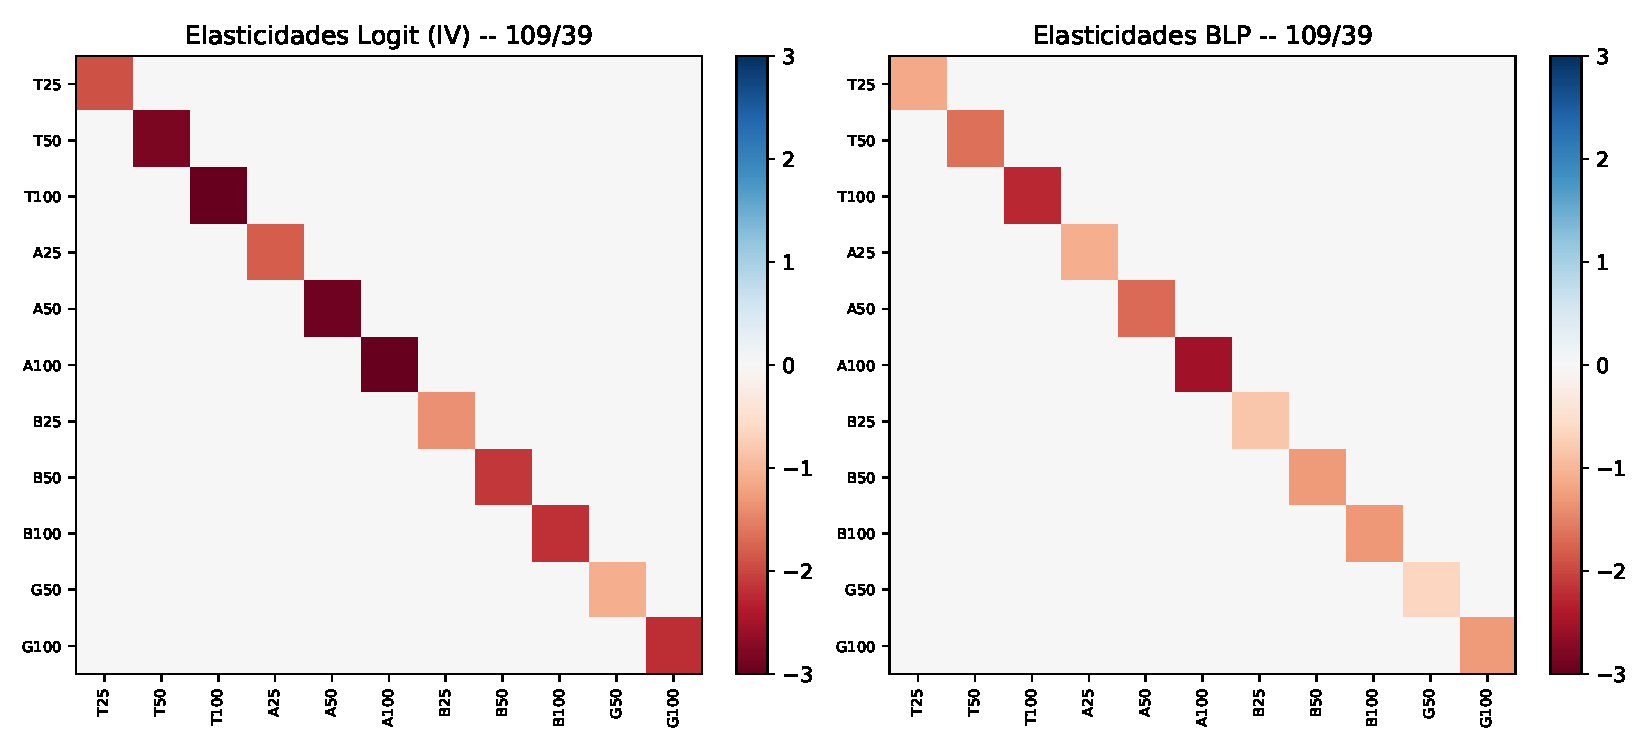
\includegraphics[width=0.85\textwidth]{../bld/fig/heatmap_elasticidades.pdf}
\caption{Matrices de elasticidades (farmacia 109, semana 39): Logit (IV) vs.\ BLP. El BLP muestra
estructura fuera de la diagonal; el Logit es esencialmente diagonal (IIA).}
\end{figure}

\begin{figure}[H]
\centering
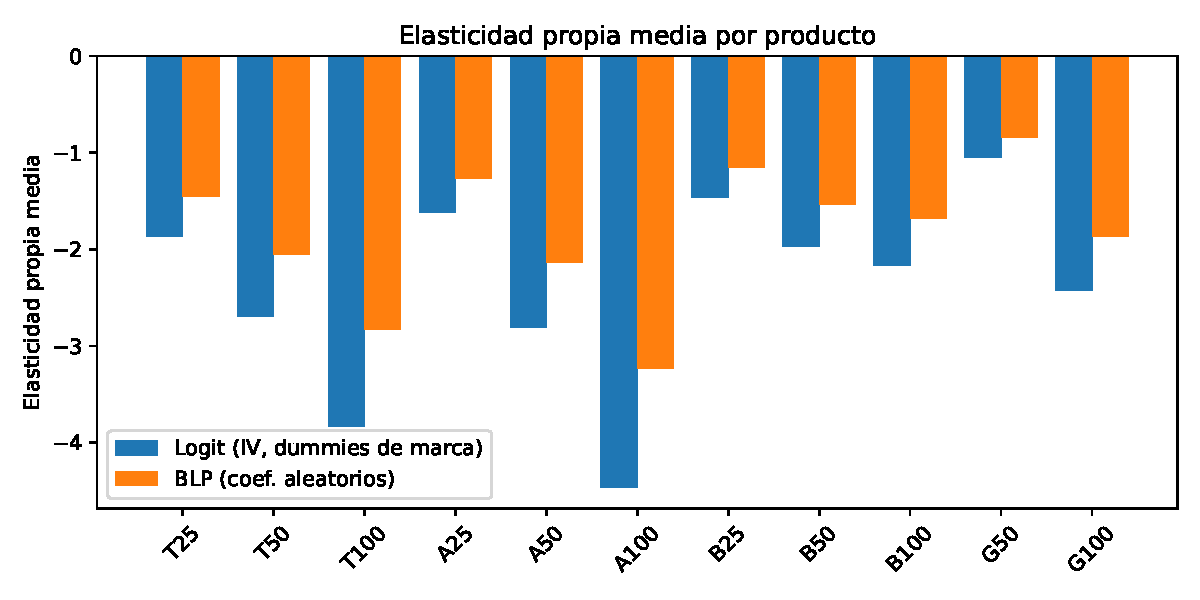
\includegraphics[width=0.7\textwidth]{../bld/fig/elas_comparacion.pdf}
\caption{Elasticidad propia media por producto: Logit (IV con dummies) vs.\ BLP.}
\end{figure}

Las elasticidades propias de BLP y del Logit IV son de magnitud comparable, pero el aporte del BLP
est\'a en las \textbf{cruzadas}: permite efectos de sustituci\'on m\'as ricos y realistas, que var\'ian
entre alternativas seg\'un su similitud (precio, marca, condici\'on de gen\'erico), en vez del patr\'on
uniforme que impone la IIA del Logit. El Nested Logit, en esta aplicaci\'on, no entrega una comparaci\'on
\'util por los problemas de identificaci\'on ya discutidos ($\hat\sigma>1$, precio positivo). Una
limitaci\'on a notar: como el bien externo concentra casi toda la cuota, la sustituci\'on hacia los
bienes internos es peque\~na; introducir un coeficiente aleatorio adicional sobre los bienes internos
relajar\'ia este punto. \\
\textit{Ver c\'odigo:} \texttt{code/hw2\_blp.py} y \texttt{code/hw2\_logit\_nl.py}.
\end{solution}

\end{questions}

\end{document}
